\section{Energy resolution boost}
\label{Result}
Assume the PE counts $N$ on a PMT with PDE $\epsilon$ for an event with visible energy $E$ obeys Poisson distribution $\pi(\lambda_N=K\epsilon E)$, in which $K$ is a factor related to light yield and detector optics. The output total charge $\sum{Q}$ is a compound Poisson random variable with the expectation $\mathrm{E}[\sum{Q}]=\lambda_N\mathrm{E}[Q]$ and variance $\mathrm{Var}[\sum{Q}]=\mathrm{E}^2[Q]\lambda_N+\lambda_N\mathrm{Var}[Q]$. The energy is estimated as $\hat{E}=\sum{Q}/(K\epsilon\mathrm{E}[Q])$ with its resolution being

\begin{equation}
    \frac{\sqrt{\mathrm{Var}[\hat{E}]}}{\mathrm{E}[\hat{E}]}=\frac{\sqrt{\mathrm{E}^2[Q]\lambda_N+\lambda_N\mathrm{Var}[Q]}}{\lambda_N\mathrm{E}[Q]}=\frac{\sqrt{1+\frac{\mathrm{Var}[Q]}{\mathrm{E}^2[Q]}}}{\sqrt{K\epsilon E}}.
\end{equation}

The PMT specific factors are $\epsilon$ (proportional to relative PDE $\epsilon^0$) and $\mathrm{Var}[Q]/ \mathrm{E}^2[Q]$ (estimated by the sample resolution $\nu^2$ in Section~\ref{sec:noisepeak}).  We plot the \emph{figure of merit} $M_{E}\equiv\sqrt{({1+\nu^2})/{\epsilon^0}}$ of the reference and nine MCP PMTs in Fig.~\ref{fig:EnergyResolution}. Besides, $1+\nu^2$ is defined as ENF in other PMT test publications~\cite{JUNOMassTesting,ENF,ENFAuger}. Despite the long tail in the charge distribution, the boost of PDE of MCP-PMTs leads to a 10\% better $M_{E}$.  Since the long tail is an undesired by-product of MCP coating to improve the collection efficiency, adopting the technology will benefit JNE overall.  We are developing an advanced waveform analysis method to model the charge distribution and count PEs that may eliminate the long-tail degradation on energy resolution.

\begin{figure}[!htbp]
    \centering
    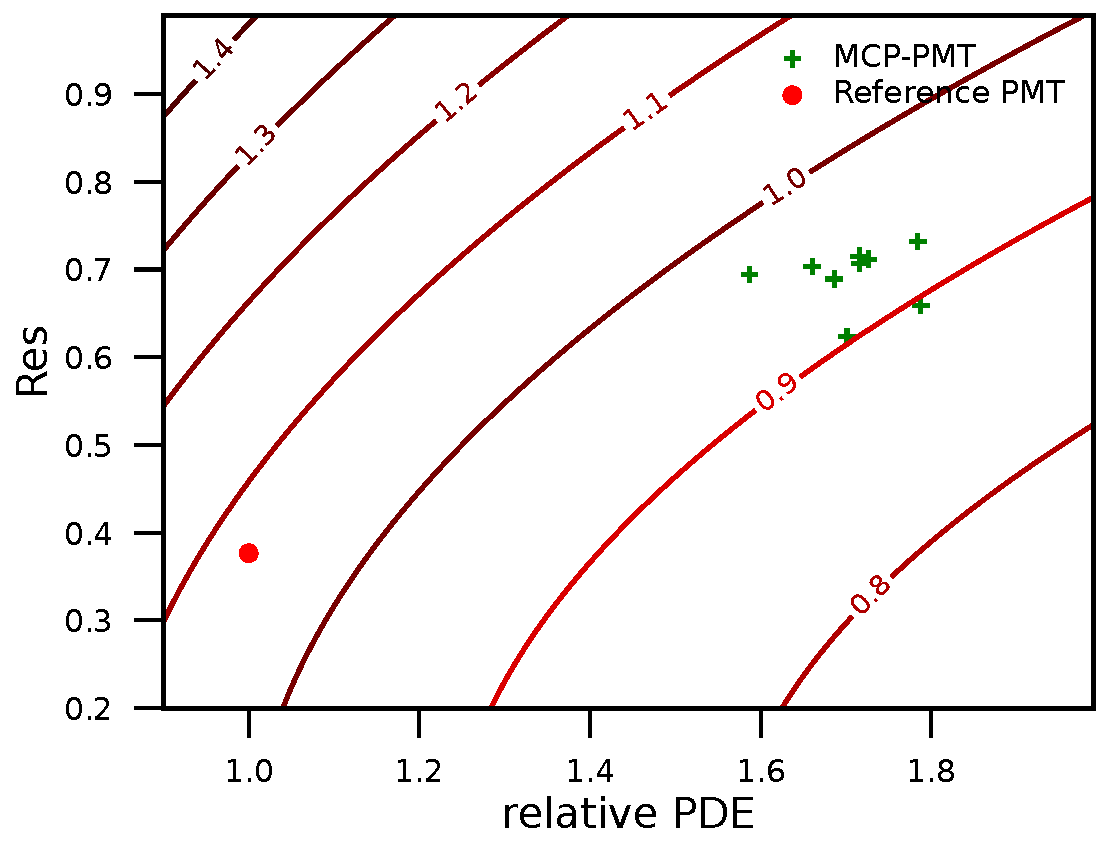
\includegraphics[width=\MF\textwidth]{figures/result/resolution.pdf}
    \caption{Contour map of energy resolution figure-of-merit $M_{E}$~(see text) as a function of the sample resolution $\nu$ and the relative PDE $\epsilon^0$. The relative PDE of the reference PMT is 1.}
    \label{fig:EnergyResolution}
\end{figure}
